%\section{Introdução}

\cappar  Como desenhar uma parábola? O famoso Galileu Galilei no seu
livro \emph{Discurso e demonstração matemática, entorno de duas novas
  ciências} (\cite{Gal14}) explicou que podemos suspender uma corrente
ligeira entre dois pregos numa parede, e esta corrente formaria uma
parábola. Na figura~\ref{fig:test} foi utilizado este procedimento.

\begin{wrapfigure}{r}{0.5\textwidth}
      \vspace{-10pt}
  \begin{figurebox}
      \centering
  \scalebox{0.35}{\Large {% GNUPLOT: LaTeX picture with Postscript
\begingroup
  \makeatletter
  \providecommand\color[2][]{%
    \GenericError{(gnuplot) \space\space\space\@spaces}{%
      Package color not loaded in conjunction with
      terminal option `colourtext'%
    }{See the gnuplot documentation for explanation.%
    }{Either use 'blacktext' in gnuplot or load the package
      color.sty in LaTeX.}%
    \renewcommand\color[2][]{}%
  }%
  \providecommand\includegraphics[2][]{%
    \GenericError{(gnuplot) \space\space\space\@spaces}{%
      Package graphicx or graphics not loaded%
    }{See the gnuplot documentation for explanation.%
    }{The gnuplot epslatex terminal needs graphicx.sty or graphics.sty.}%
    \renewcommand\includegraphics[2][]{}%
  }%
  \providecommand\rotatebox[2]{#2}%
  \@ifundefined{ifGPcolor}{%
    \newif\ifGPcolor
    \GPcolorfalse
  }{}%
  \@ifundefined{ifGPblacktext}{%
    \newif\ifGPblacktext
    \GPblacktexttrue
  }{}%
  % define a \g@addto@macro without @ in the name:
  \let\gplgaddtomacro\g@addto@macro
  % define empty templates for all commands taking text:
  \gdef\gplbacktext{}%
  \gdef\gplfronttext{}%
  \makeatother
  \ifGPblacktext
    % no textcolor at all
    \def\colorrgb#1{}%
    \def\colorgray#1{}%
  \else
    % gray or color?
    \ifGPcolor
      \def\colorrgb#1{\color[rgb]{#1}}%
      \def\colorgray#1{\color[gray]{#1}}%
      \expandafter\def\csname LTw\endcsname{\color{white}}%
      \expandafter\def\csname LTb\endcsname{\color{black}}%
      \expandafter\def\csname LTa\endcsname{\color{black}}%
      \expandafter\def\csname LT0\endcsname{\color[rgb]{1,0,0}}%
      \expandafter\def\csname LT1\endcsname{\color[rgb]{0,1,0}}%
      \expandafter\def\csname LT2\endcsname{\color[rgb]{0,0,1}}%
      \expandafter\def\csname LT3\endcsname{\color[rgb]{1,0,1}}%
      \expandafter\def\csname LT4\endcsname{\color[rgb]{0,1,1}}%
      \expandafter\def\csname LT5\endcsname{\color[rgb]{1,1,0}}%
      \expandafter\def\csname LT6\endcsname{\color[rgb]{0,0,0}}%
      \expandafter\def\csname LT7\endcsname{\color[rgb]{1,0.3,0}}%
      \expandafter\def\csname LT8\endcsname{\color[rgb]{0.5,0.5,0.5}}%
    \else
      % gray
      \def\colorrgb#1{\color{black}}%
      \def\colorgray#1{\color[gray]{#1}}%
      \expandafter\def\csname LTw\endcsname{\color{white}}%
      \expandafter\def\csname LTb\endcsname{\color{black}}%
      \expandafter\def\csname LTa\endcsname{\color{black}}%
      \expandafter\def\csname LT0\endcsname{\color{black}}%
      \expandafter\def\csname LT1\endcsname{\color{black}}%
      \expandafter\def\csname LT2\endcsname{\color{black}}%
      \expandafter\def\csname LT3\endcsname{\color{black}}%
      \expandafter\def\csname LT4\endcsname{\color{black}}%
      \expandafter\def\csname LT5\endcsname{\color{black}}%
      \expandafter\def\csname LT6\endcsname{\color{black}}%
      \expandafter\def\csname LT7\endcsname{\color{black}}%
      \expandafter\def\csname LT8\endcsname{\color{black}}%
    \fi
  \fi
  \setlength{\unitlength}{0.0500bp}%
  \begin{picture}(11520.00,8640.00)%
    \gplgaddtomacro\gplbacktext{%
      \colorrgb{0.00,0.00,0.00}%
      \put(300,400){\makebox(0,0)[r]{\strut{}1}}%
      \colorrgb{0.00,0.00,0.00}%
      \put(300,2000){\makebox(0,0)[r]{\strut{}2}}%
      \colorrgb{0.00,0.00,0.00}%
      \put(300,3600){\makebox(0,0)[r]{\strut{}3}}%
      \colorrgb{0.00,0.00,0.00}%
      \put(300,5199){\makebox(0,0)[r]{\strut{}4}}%
      \colorrgb{0.00,0.00,0.00}%
      \put(300,6799){\makebox(0,0)[r]{\strut{}5}}%
      \colorrgb{0.00,0.00,0.00}%
      \put(300,8399){\makebox(0,0)[r]{\strut{}6}}%
      \colorrgb{0.00,0.00,0.00}%
      \put(864,200){\makebox(0,0){\strut{}-1}}%
      \colorrgb{0.00,0.00,0.00}%
      \put(1975,200){\makebox(0,0){\strut{}-0.5}}%
      \colorrgb{0.00,0.00,0.00}%
      \put(3086,200){\makebox(0,0){\strut{}0}}%
      \colorrgb{0.00,0.00,0.00}%
      \put(4197,200){\makebox(0,0){\strut{}0.5}}%
      \colorrgb{0.00,0.00,0.00}%
      \put(5308,200){\makebox(0,0){\strut{}1}}%
      \colorrgb{0.00,0.00,0.00}%
      \put(6419,200){\makebox(0,0){\strut{}1.5}}%
      \colorrgb{0.00,0.00,0.00}%
      \put(7530,200){\makebox(0,0){\strut{}2}}%
      \colorrgb{0.00,0.00,0.00}%
      \put(8640,200){\makebox(0,0){\strut{}2.5}}%
      \colorrgb{0.00,0.00,0.00}%
      \put(9751,200){\makebox(0,0){\strut{}3}}%
      \colorrgb{0.00,0.00,0.00}%
      \put(10862,200){\makebox(0,0){\strut{}3.5}}%
    }%
    \gplgaddtomacro\gplfronttext{%
      \colorrgb{0.00,0.00,0.00}%
      \put(9529,6799){\makebox(0,0){\Huge \bf S}}%
      \put(1975,1520){\makebox(0,0){\Huge $T_0$}}%
      \put(2642,1520){\makebox(0,0){\Huge\bf I}}%
      \put(5752,2000){\makebox(0,0){\Huge $F_x$}}%
      \put(7530,3120){\makebox(0,0){\Huge $T_x$}}%
      \put(5308,3440){\makebox(0,0){\Huge $P=(x,y)$}}%
    }%
    \gplbacktext
    \put(0,0){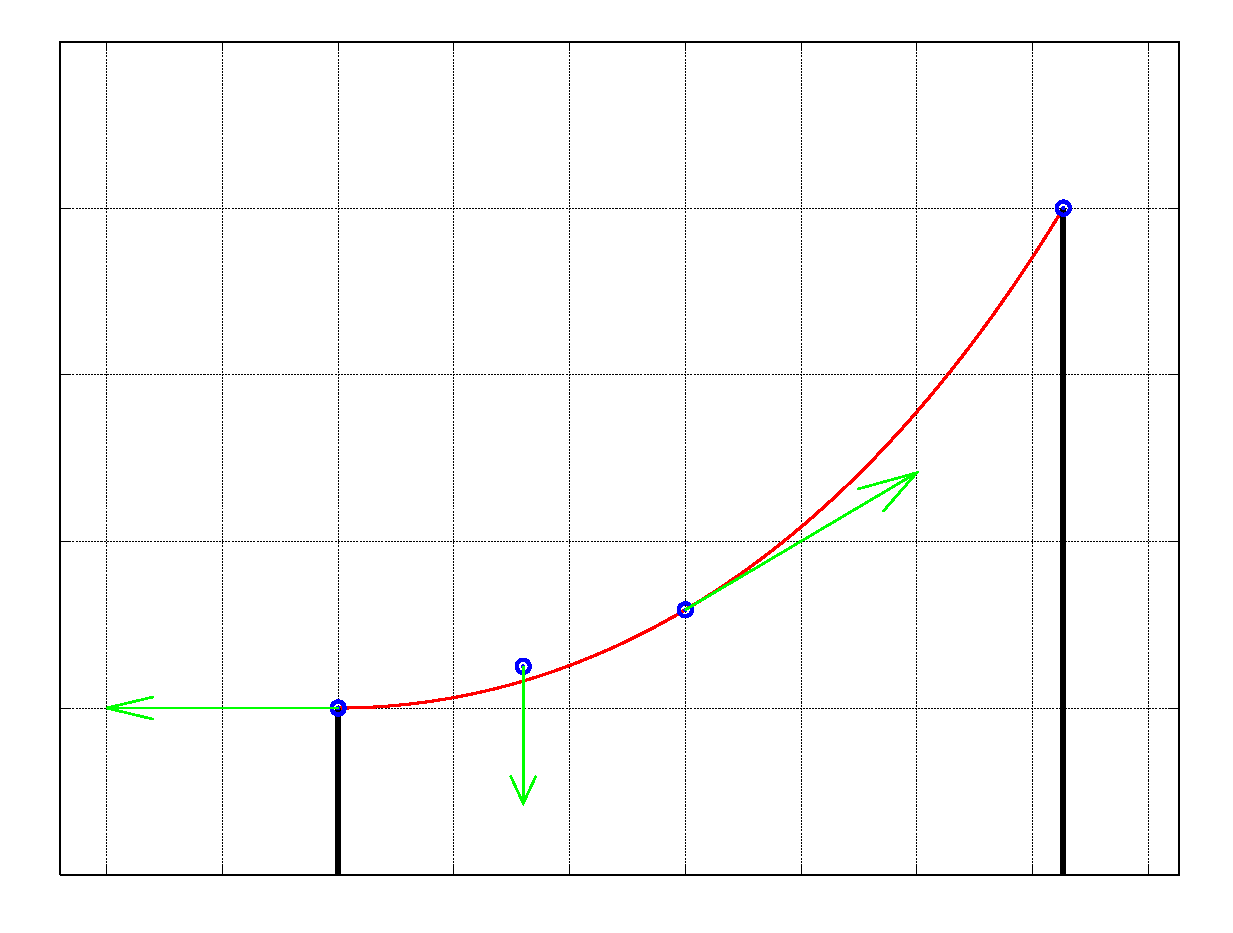
\includegraphics{catenaria_con_fuerzas}}%
    \gplfronttext
  \end{picture}%
\endgroup
}}
  \caption{Forças que atuam sobre o segmento de catenária entre pontos $I$ e $P$.}
    \label{fig:1}
  \end{figurebox}
      \vspace{-40pt}
\end{wrapfigure}
%\marginnote{\scalebox{0.1}{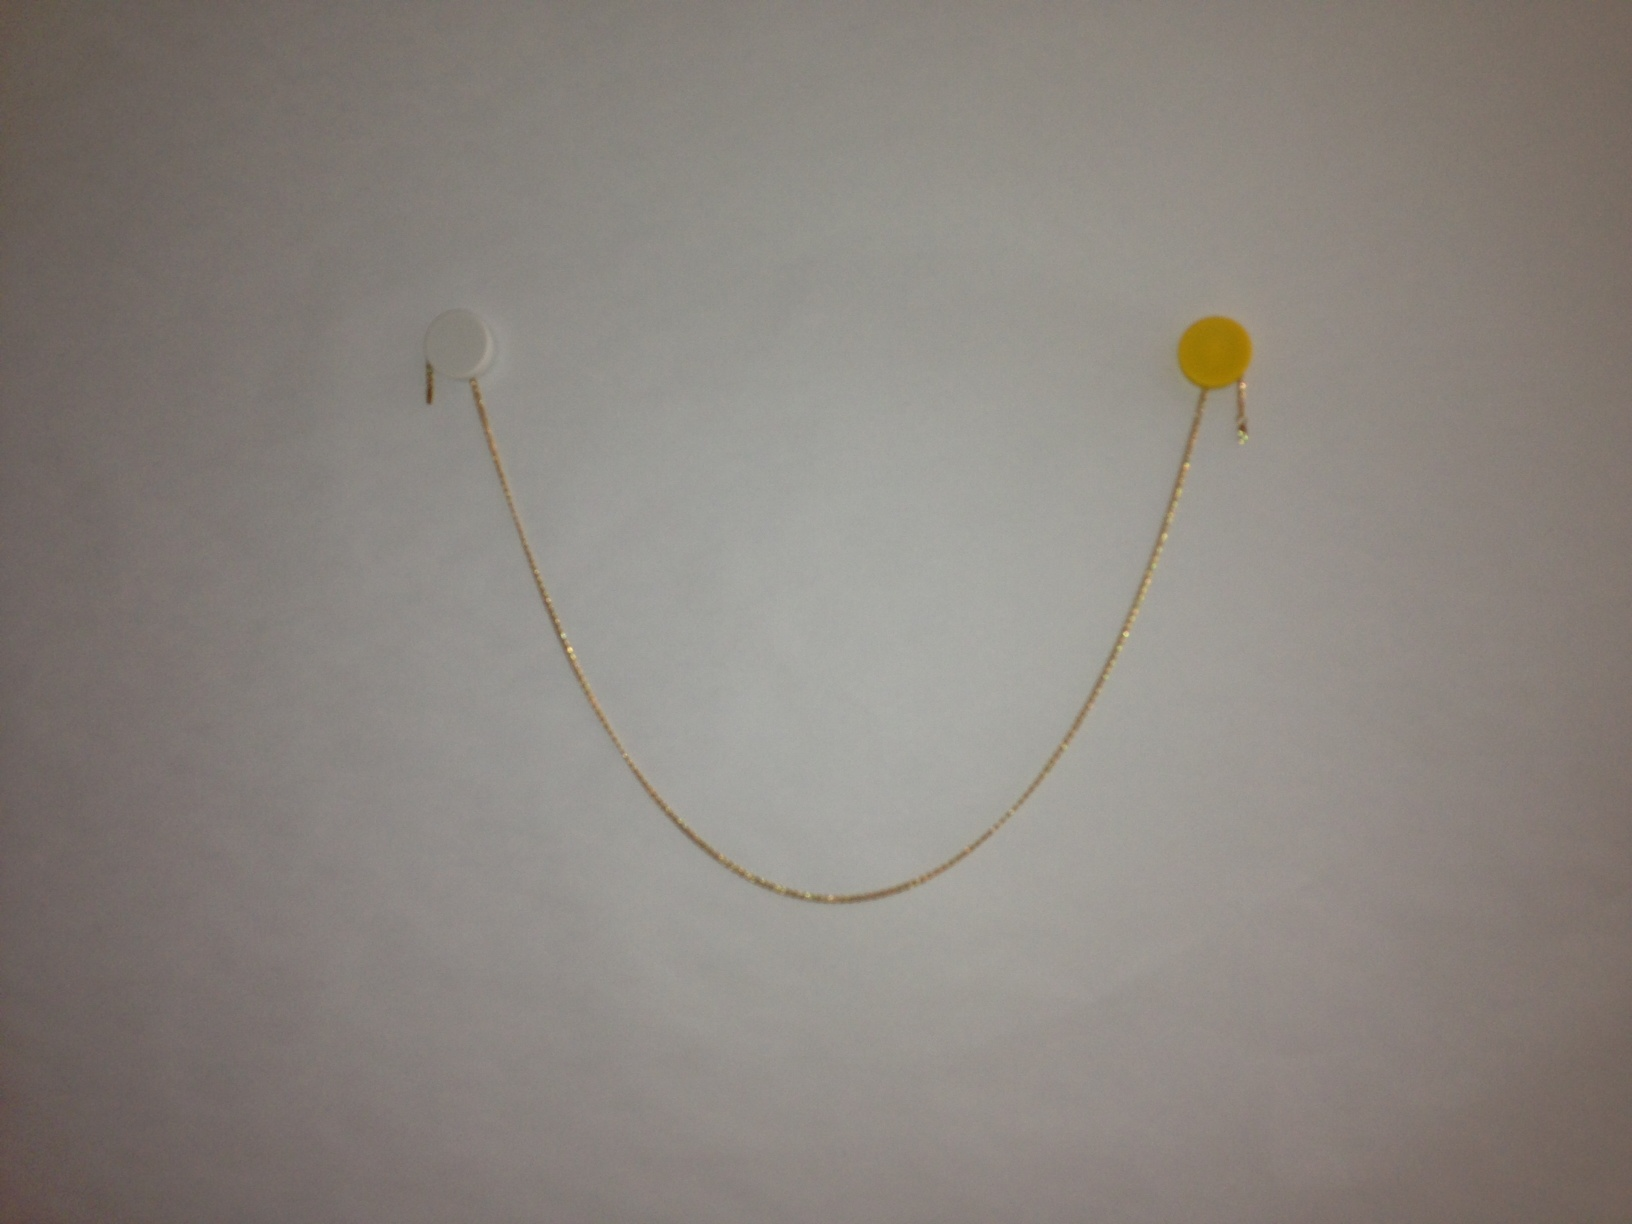
\includegraphics{i2.jpeg}}}
\vspace{0.5cm}
O que obtemos é bastante parecido com uma parábola, mas não é. A
curva chama-se \emph{catenária} e vamos ver como podemos corrigir o
erro de Galileu e encontrar a fórmula que define esta curva.

\section{Forças}
Em primeiro lugar, temos que fazer algumas suposições. Em lugar de considerar
uma corrente, consideramos uma linha com massa distribuída uniformemente. A
linha suspensa entre dois postes como na figura~\ref{fig:1}, em que
a desenhámos em cor vermelha e os postes estão marcados em
preto. Vamos supor que a linha está tangente à reta horizontal no
ponto $I$ do lado esquerdo onde está fixada. Podemos supor que
a coordenada abscissa do ponto $I$ é igual a $0.$




Porque podemos supor que no ponto $I$ a linha é tangente a uma
reta horizontal? Ilustramo-lo na foto~\ref{fig:test}. A
demonstração deste facto será clara, quando se entender como atuam
as forças sobre a linha.

\begin{wrapfigure}{r}{0.5\textwidth}
  \vspace{-12pt}
  \begin{figurebox}
      \centering
  \begin{tikzpicture}
    \draw [->, very thick, bluesol] (0,0) -- (6,0);
    \draw [bluesol] (3,-0.4) node {$T_0$};
    \draw [->, very thick, bluesol] (0,0) -- (0,2);
    \draw [bluesol] (-0.4,1) node {$F_x$};
    \draw [->, very thick, newgreen] (0,0) -- (6,2);
    \draw [newgreen] (4.5,1) node {$T_x$};
    \draw (0,-0.4) node {$P=(x,y)$};
    \draw [dotted, graysol] (0,2) -- (6,2);
    \draw [dotted, graysol] (6,0) -- (6,2);
    \draw [redsol, thick] (0,0) .. controls (2,0.8) and (2.5 , 1.2) .. (4,2.5);
    \draw [graysol, very  thick] (3,0) arc (0:18.435:3);
    \draw (2,0.3) node {$\alpha$};
    \draw [fill=black] (0,0) circle (0.1 );
  \end{tikzpicture}
  \caption{as forças juntos.}
  \label{fig:2}
  \end{figurebox}
  \vspace{-10pt}
\end{wrapfigure}

Agora escolhemos um ponto $P=(x,y)$ na linha entre pontos de fixação
$I$ e $S$. Consideramos a parte de linha entre os pontos $I$ e
$P$. A tensão $\vec{T}_0$ da linha no ponto $I$ é horizontal, uma vez
que a linha é perpendicular ao poste neste ponto. Chamamo-la
$\vec{T}_0$ para marcar que é a tensão no ponto com coordenada
$x=0$. A magnitude desta força (que é igual à longitude deste
vetor) denotamo-la por $T_0$.

No outro extremo do segmento da linha, a tensão é distinta, ou seja,
no ponto $P$ na figura~\ref{fig:1}. Isso é uma consequência do
facto que o segmento pesa. A tensão denotamo-la por $\vec{T}_x$, o
peso por $\vec{F}_x$ e as suas magnitudes por $T_x$ e $F_x$
respetivamente. Na figura~\ref{fig:1} o vetor do peso foi
colocado no centro de massa da linha.

Estas são as únicas forças que atuam sobre o segmento da linha entre
$I$ e $P$. Como a linha não se move da segunda lei de Newton,
temos que a soma vetorial das forças é igual a $0$. Isto é
\begin{displaymath}
  \vec{T}_0+\vec{T}_x+\vec{F}=0.
\end{displaymath}
Para comparar as magnitudes dos vetores em figura~\ref{fig:2}
colocamo-los no ponto $P$ e mudamos as direções do $\vec{T}_0$
e $\vec{F}$.


\begin{wrapfigure}{r}{0.5\textwidth}
  \begin{mybox}
    A palavra \emph{catenária} procede da palavra \emph{catena},
    que significa \emph{corrente} em Latim.
\end{mybox}
\end{wrapfigure}
Portanto, utilizando esta figura podemos escrever as seguintes
equações matemáticas.
\begin{equation}
  \label{eq:7}
  \left\{
    \begin{array}{l}
      T_x\cos(\alpha) = T_0 \\
      T_x\sin(\alpha) = F_x.
    \end{array}
\right.
\end{equation}

Se entender donde vêm estas fórmulas, parabéns. Caso contrário, por favor não se sinta mal. Entender como atuam forças sobre um
segmento de linha não é fácil e requer tempo. Recomendamos-lhe
analisar as figuras~\ref{fig:1} e~\ref{fig:2} e ler de novo esta
seção.


\begin{figure}
  \begin{figurebox}
    \vspace{20pt}
    \centering
\begin{subfigure}{.5\textwidth}
  \centering
   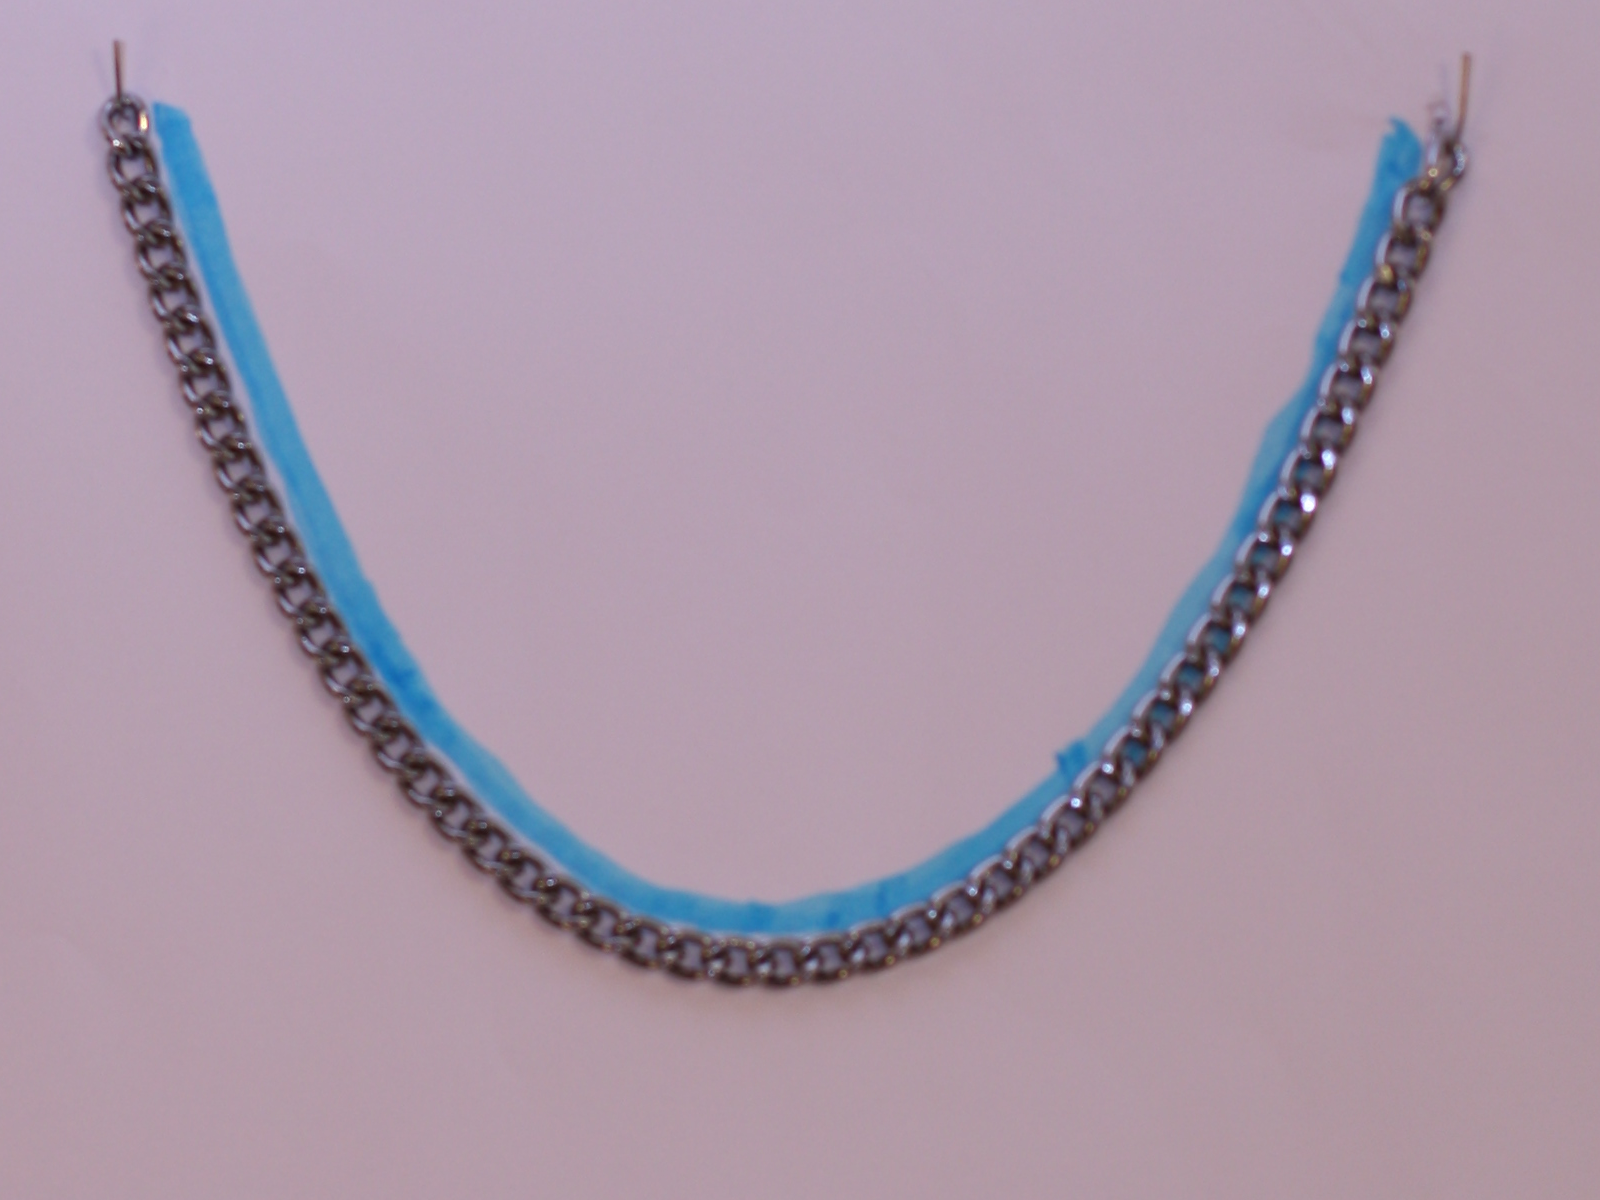
\includegraphics[height=130pt]{cat1.png}
   \caption{}
  \label{fig:0a}
\end{subfigure}%
\begin{subfigure}{.5\textwidth}
  \centering
  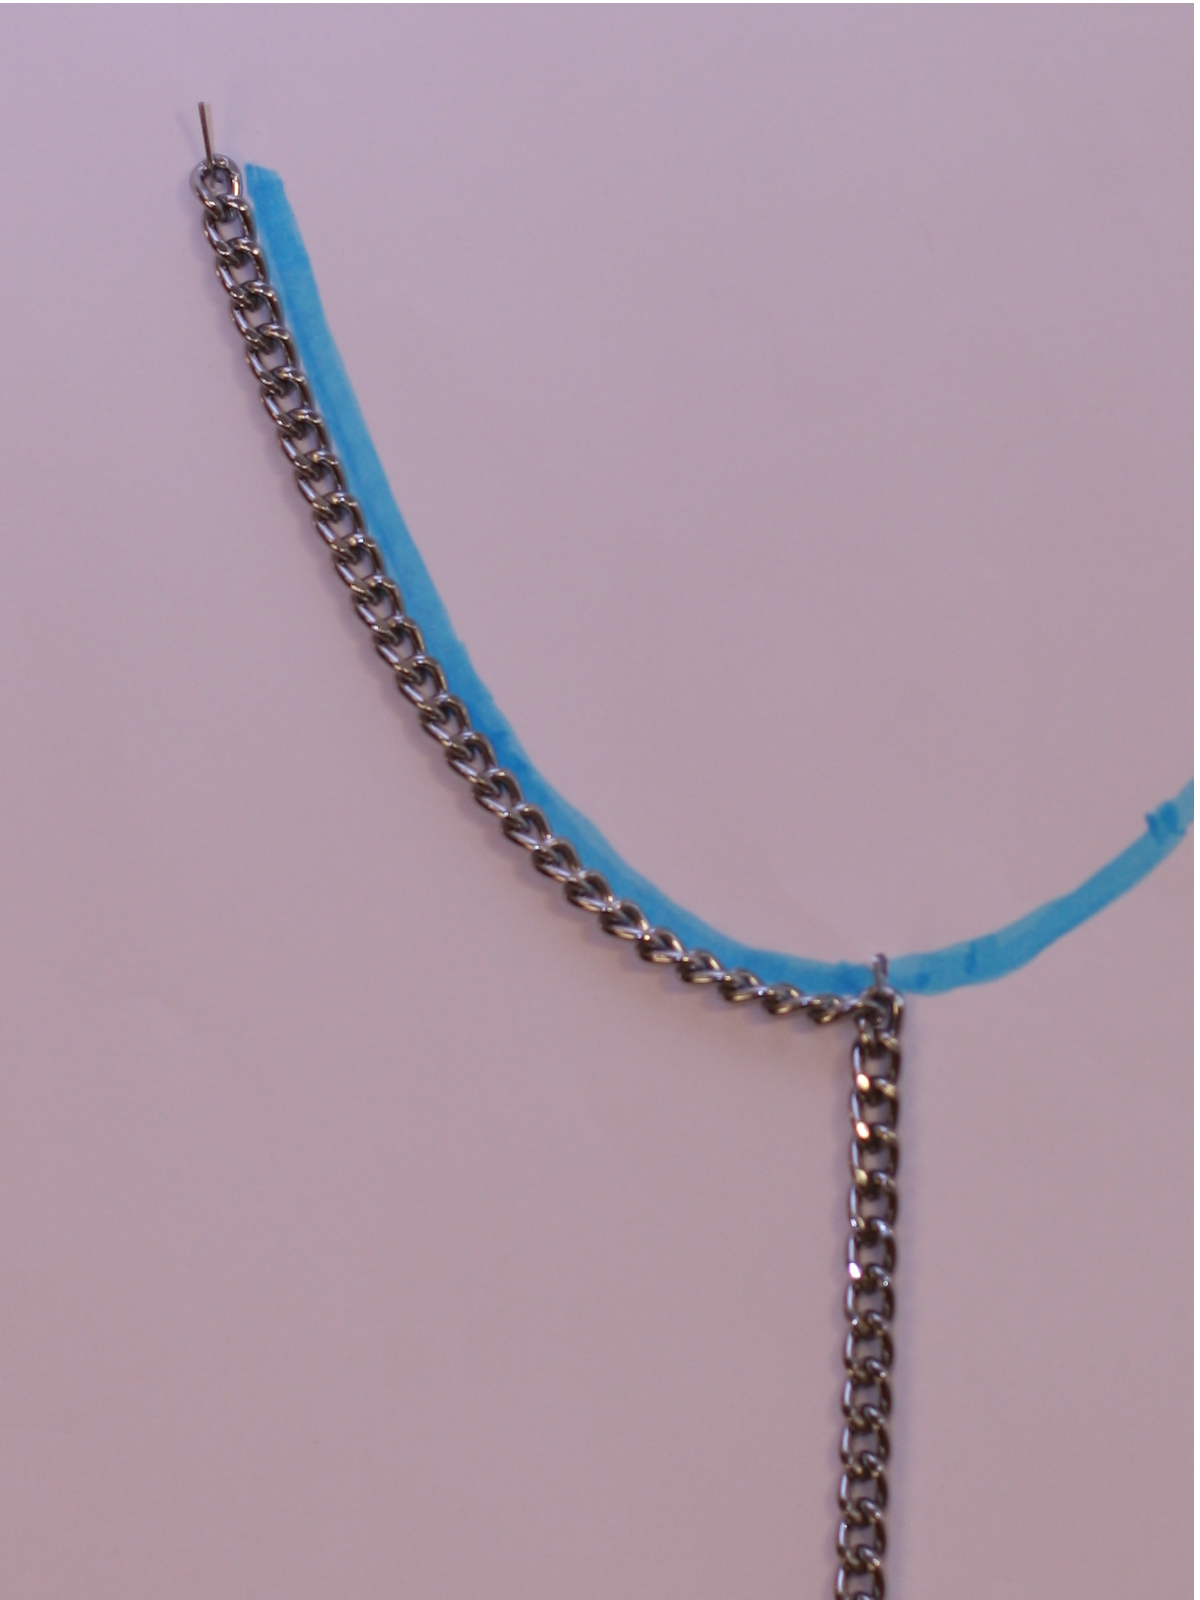
\includegraphics[width=130pt]{cat2.png}
  \caption{}
  \label{fig:0b}
\end{subfigure}
\caption{Uma corrente ligeira.}
\label{fig:test}
  \end{figurebox}
\end{figure}


\section{A fórmula da catenária}

O nosso objetivo é encontrar a fórmula da catenária. O que é que isso significa? Isso significa que queremos encontrar uma função $y=f(x)$ que o
seu gráfico é a curva vermelha em figura~\ref{fig:1}. Como podemos
fazê-lo? Claramente vamos utilizar as equações em
(\ref{eq:7}). Mas em (\ref{eq:7}) não há nenhum $y$ e $x$ é um
índice não variável? Portanto, a questão é procurar a derivada de $f$ e
depois integrá-la. Ah, ah, ah, mas, (\ref{eq:7}) também não tem derivada.
Pois, tem, mas não explicitamente.



 Recordamos, que a derivada de
uma função $f$ num ponto $x$ é a pendente da reta tangente
ao gráfico de $f$ no ponto $x$. Podemos denotá-la por $f'(x)$ ou por
$dy/dx$. Isto é
\begin{displaymath}
  \frac{dy}{dx}=f'(x)=\tan(\alpha)=\frac{\sin(\alpha)}{\cos(\alpha)}.
\end{displaymath}
Então, dividindo a primeira equação em (\ref{eq:7}) pela segunda, vamos obter que
\begin{equation}
  \label{eq:8}
  \frac{dy}{dx}=\frac{F_x}{T_0}.
\end{equation}

Na ultima equação $T_0$ é um valor que não depende da variável
$x$, e portanto não complica. O que temos que averiguar é,
portanto, quanto é $F_x$. Primeiro, vamos supor que a relação
entre $x$ e a força $F_x$ é linear. Como vamos ver mais tarde, esta
suposição não é correta, mas permite-nos chegar à mesma
conclusão à qual chegaram Leonardo Da Vinci e Galileu entre outros, que a
curva é uma parábola.


\begin{wrapfigure}{r}{0.7\textwidth}
  \begin{figurebox}
      \centering
  \scalebox{0.57}{% GNUPLOT: LaTeX picture with Postscript
\begingroup
  \makeatletter
  \providecommand\color[2][]{%
    \GenericError{(gnuplot) \space\space\space\@spaces}{%
      Package color not loaded in conjunction with
      terminal option `colourtext'%
    }{See the gnuplot documentation for explanation.%
    }{Either use 'blacktext' in gnuplot or load the package
      color.sty in LaTeX.}%
    \renewcommand\color[2][]{}%
  }%
  \providecommand\includegraphics[2][]{%
    \GenericError{(gnuplot) \space\space\space\@spaces}{%
      Package graphicx or graphics not loaded%
    }{See the gnuplot documentation for explanation.%
    }{The gnuplot epslatex terminal needs graphicx.sty or graphics.sty.}%
    \renewcommand\includegraphics[2][]{}%
  }%
  \providecommand\rotatebox[2]{#2}%
  \@ifundefined{ifGPcolor}{%
    \newif\ifGPcolor
    \GPcolorfalse
  }{}%
  \@ifundefined{ifGPblacktext}{%
    \newif\ifGPblacktext
    \GPblacktexttrue
  }{}%
  % define a \g@addto@macro without @ in the name:
  \let\gplgaddtomacro\g@addto@macro
  % define empty templates for all commands taking text:
  \gdef\gplbacktext{}%
  \gdef\gplfronttext{}%
  \makeatother
  \ifGPblacktext
    % no textcolor at all
    \def\colorrgb#1{}%
    \def\colorgray#1{}%
  \else
    % gray or color?
    \ifGPcolor
      \def\colorrgb#1{\color[rgb]{#1}}%
      \def\colorgray#1{\color[gray]{#1}}%
      \expandafter\def\csname LTw\endcsname{\color{white}}%
      \expandafter\def\csname LTb\endcsname{\color{black}}%
      \expandafter\def\csname LTa\endcsname{\color{black}}%
      \expandafter\def\csname LT0\endcsname{\color[rgb]{1,0,0}}%
      \expandafter\def\csname LT1\endcsname{\color[rgb]{0,1,0}}%
      \expandafter\def\csname LT2\endcsname{\color[rgb]{0,0,1}}%
      \expandafter\def\csname LT3\endcsname{\color[rgb]{1,0,1}}%
      \expandafter\def\csname LT4\endcsname{\color[rgb]{0,1,1}}%
      \expandafter\def\csname LT5\endcsname{\color[rgb]{1,1,0}}%
      \expandafter\def\csname LT6\endcsname{\color[rgb]{0,0,0}}%
      \expandafter\def\csname LT7\endcsname{\color[rgb]{1,0.3,0}}%
      \expandafter\def\csname LT8\endcsname{\color[rgb]{0.5,0.5,0.5}}%
    \else
      % gray
      \def\colorrgb#1{\color{black}}%
      \def\colorgray#1{\color[gray]{#1}}%
      \expandafter\def\csname LTw\endcsname{\color{white}}%
      \expandafter\def\csname LTb\endcsname{\color{black}}%
      \expandafter\def\csname LTa\endcsname{\color{black}}%
      \expandafter\def\csname LT0\endcsname{\color{black}}%
      \expandafter\def\csname LT1\endcsname{\color{black}}%
      \expandafter\def\csname LT2\endcsname{\color{black}}%
      \expandafter\def\csname LT3\endcsname{\color{black}}%
      \expandafter\def\csname LT4\endcsname{\color{black}}%
      \expandafter\def\csname LT5\endcsname{\color{black}}%
      \expandafter\def\csname LT6\endcsname{\color{black}}%
      \expandafter\def\csname LT7\endcsname{\color{black}}%
      \expandafter\def\csname LT8\endcsname{\color{black}}%
    \fi
  \fi
  \setlength{\unitlength}{0.0500bp}%
  \begin{picture}(11520.00,8640.00)%
    \gplgaddtomacro\gplbacktext{%
      \colorrgb{0.00,0.00,0.00}%
      \put(300,400){\makebox(0,0)[r]{\strut{}0}}%
      \colorrgb{0.00,0.00,0.00}%
      \put(300,2000){\makebox(0,0)[r]{\strut{}1}}%
      \colorrgb{0.00,0.00,0.00}%
      \put(300,3600){\makebox(0,0)[r]{\strut{}2}}%
      \colorrgb{0.00,0.00,0.00}%
      \put(300,5199){\makebox(0,0)[r]{\strut{}3}}%
      \colorrgb{0.00,0.00,0.00}%
      \put(300,6799){\makebox(0,0)[r]{\strut{}4}}%
      \colorrgb{0.00,0.00,0.00}%
      \put(300,8399){\makebox(0,0)[r]{\strut{}5}}%
      \colorrgb{0.00,0.00,0.00}%
      \put(420,200){\makebox(0,0){\strut{}-4}}%
      \colorrgb{0.00,0.00,0.00}%
      \put(1762,200){\makebox(0,0){\strut{}-3}}%
      \colorrgb{0.00,0.00,0.00}%
      \put(3105,200){\makebox(0,0){\strut{}-2}}%
      \colorrgb{0.00,0.00,0.00}%
      \put(4447,200){\makebox(0,0){\strut{}-1}}%
      \colorrgb{0.00,0.00,0.00}%
      \put(5790,200){\makebox(0,0){\strut{}0}}%
      \colorrgb{0.00,0.00,0.00}%
      \put(7132,200){\makebox(0,0){\strut{}1}}%
      \colorrgb{0.00,0.00,0.00}%
      \put(8474,200){\makebox(0,0){\strut{}2}}%
      \colorrgb{0.00,0.00,0.00}%
      \put(9817,200){\makebox(0,0){\strut{}3}}%
      \colorrgb{0.00,0.00,0.00}%
      \put(11159,200){\makebox(0,0){\strut{}4}}%
    }%
    \gplgaddtomacro\gplfronttext{%
      \csname LTb\endcsname%
      \put(10256,4799){\makebox(0,0){h=0.5}}%
      \csname LTb\endcsname%
      \put(10256,4599){\makebox(0,0){h=1}}%
      \csname LTb\endcsname%
      \put(10256,4399){\makebox(0,0){h=1.5}}%
      \csname LTb\endcsname%
      \put(10256,4199){\makebox(0,0){h=2}}%
      \csname LTb\endcsname%
      \put(10256,3999){\makebox(0,0){h=2.5}}%
    }%
    \gplbacktext
    \put(0,0){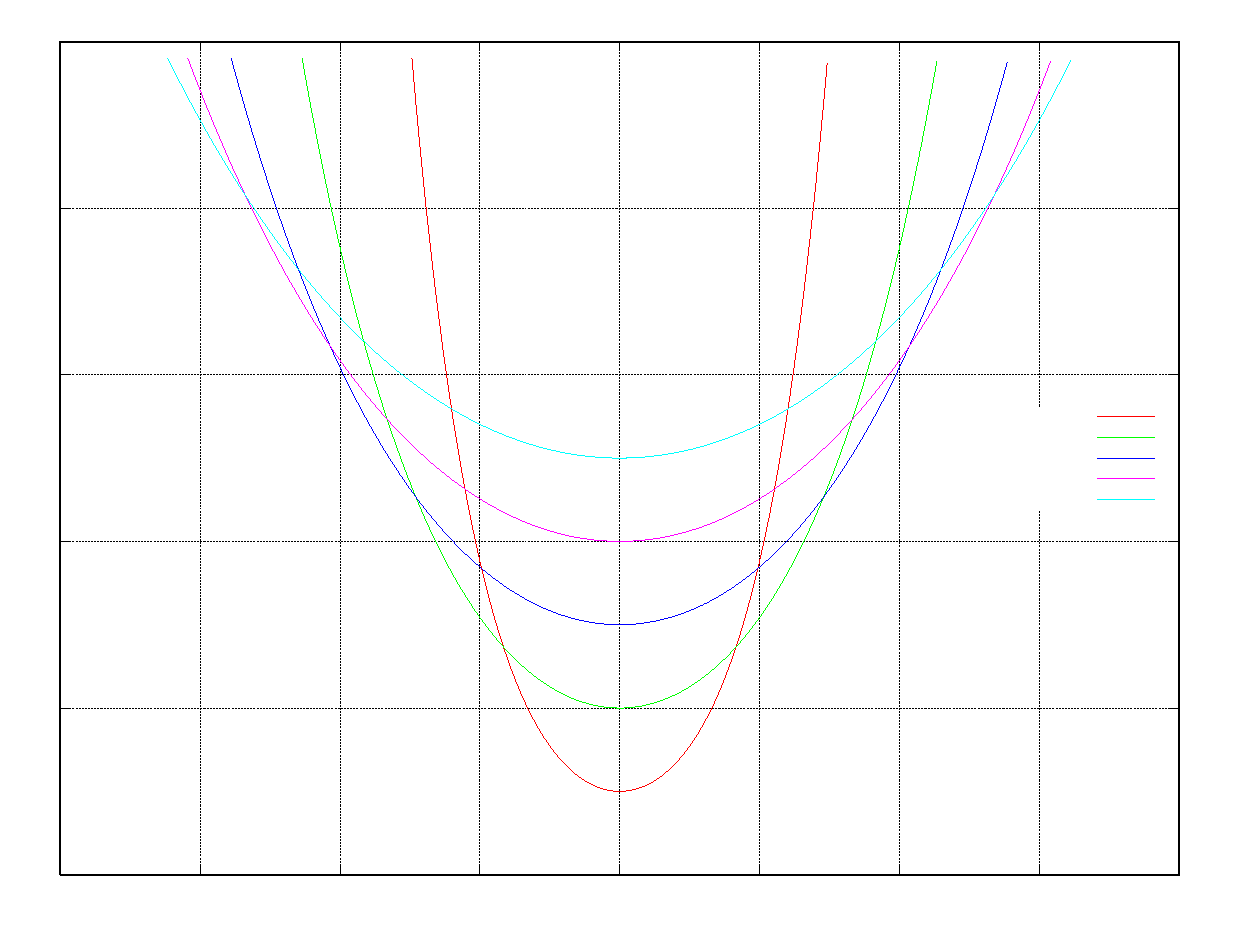
\includegraphics{catenaria_estandard_con_diferente_a}}%
    \gplfronttext
  \end{picture}%
\endgroup
}
  \caption{Função $f(x)=h \cosh(x/h)$ para
    $h = 0.5, 1, 1.5, 2, 2.5$.}
  \label{fig:15}
  \end{figurebox}
  \vspace{5pt}
\end{wrapfigure}

Então, vamos supor que $F_x$ é proporcional a $x$. Isto é $F_x= k x
$ em que $k$ é uma constante que não conhecemos. Portanto, a
equação \eqref{eq:8} reescreve-se como
\begin{displaymath}
  \frac{dy}{dx}=\frac{k x}{T_0}
\end{displaymath}
e para averiguar quanto é $y=f(x)$ é suficiente integrar esta
equação. Então
\begin{displaymath}
  e= \frac{x^2}{2b}+c,
\end{displaymath}
em que $b=T_0/k$ e isto é uma parábola.


A fórmula que obtivemos em muitos casos, não está muito longe da
realidade, mas não é correta. Não é certo que o peso do segmento
da linha entre $I$ e $P=(x,y)$ é proporcional a $x$.  Se o pensarmos,
o peso tem que ser proporcional à longitude $l$ do segmento. De
facto é igual a $g \lambda l$, em que $\lambda$ é o valor do peso
por unidade de longitude e $g$ é a aceleração devida à
gravitação. Então, a equação (\ref{eq:8}) dá uma fórmula um
pouco diferente
\begin{equation}
  \label{eq:9}
  \frac{dy}{dx}=\frac{g \lambda l}{T_0}=\frac{l}{a},
\end{equation}
em que substituímos $\frac{T_0}{g \lambda}$ por uma constante $a$.

Portanto, para encontrar a fórmula para $y$ temos que saber
como calcular a longitude $l$. Isso vamos explicá-lo um pouco na
seguinte seçção. O mais importante, por enquanto, é a seguinte
equação diferencial que nos permite relacionar a derivada de $l$
com a derivada de $y$,
\begin{equation}
  \label{eq:4}
  \frac{dl}{dx}=\sqrt{1+\Big(\frac{dy}{dx}\Big)^2}.
\end{equation}
Por outra parte $dl/dx$ podemos calculá-lo diferenciando ambos os lados do
(\ref{eq:9}) relativamente a $x$, isto é
\begin{displaymath}
  \frac{d^2y}{dx^2}=\frac{1}{a}\frac{dl}{dx}
\end{displaymath}
e portanto substituindo em (\ref{eq:4}) temos a seguinte
equação diferencial
\begin{displaymath}
  \sqrt{1+\Big(\frac{dy}{dx}\Big)^2}=a\frac{d^2y}{dx^2}.
\end{displaymath}

\begin{wrapfigure}{r}{0.5\textwidth}
  \begin{mybox}
    \centering
    \emph{\textcolor{bluesol}{Seno e cosseno hiperbólico}}
    \begin{align*}
      &\senh(x)=\frac{e^x-e^{-x}}{2}\\
      &\cosh(x)=\frac{e^x+e^{-x}}{2}\\
      &\senh'(x)=\frac{e^x+e^{-x}}{2}=\cosh(x)\\
      &\cosh'(x)=\senh(x)\\
      &\senh^2(x)+\cosh^2(x)=-1.
    \end{align*}
    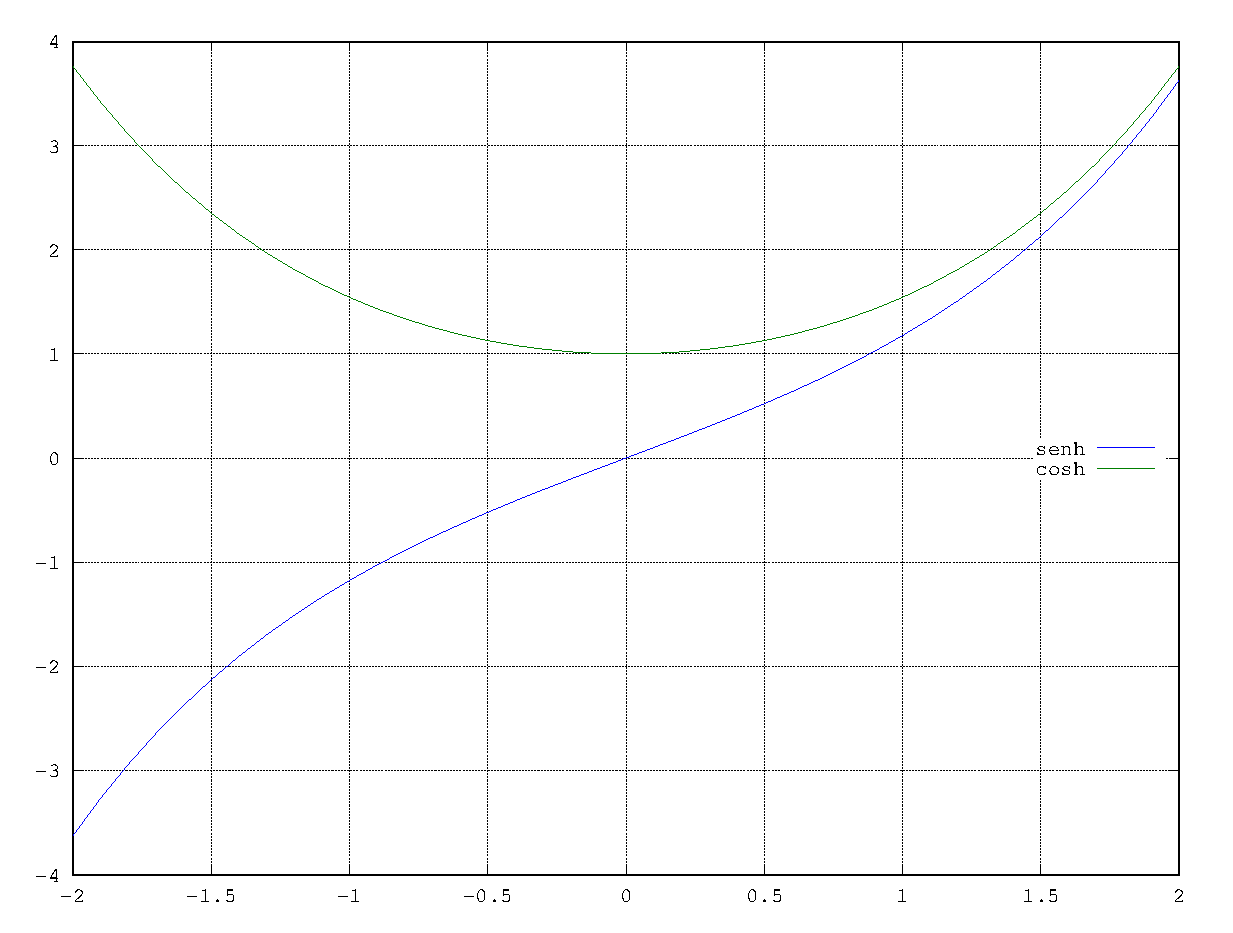
\includegraphics[width=\columnwidth]{shch}
  \end{mybox}
  \vspace{1cm}
\end{wrapfigure}

Agora, para resolver esta última que pode parecer complicada, vamos
introduzir uma nova variável $z=dy/dx$. Então $dz/dx={d^2y}/{dx^2}$ e
temos que
\begin{displaymath}
  \sqrt{1+z^2}=a\frac{dz}{dx}.
\end{displaymath}
Isto é uma equação diferencial que podemos resolver separando as
variáveis. Com efeito, primeiro separamos $x$ e $z$,
\begin{displaymath}
  \frac{dx}{a}=\frac{dz}{\sqrt{1+z^2}},
\end{displaymath}
e depois integramos
\begin{displaymath}
  \frac{x}{a}=\int\frac{dz}{\sqrt{1+z^2}}=\arsenh(z)+c_1.
\end{displaymath}
Então $z=\senh(x/a-c_1)$ e como $z=dy/dx$
\begin{displaymath}
  y=\int \senh(x/a-c_1) dx = a\cosh(x/a-c_1) + c_2.
\end{displaymath}
Esta solução reescrevemo-la como
\begin{equation}
    \label{eq:5}
    \boxed{y= a\cosh\Big(\frac{x-C_1}{a}\Big) + C_2.}
\end{equation}


\begin{wrapfigure}{l}{0.5\textwidth}
\begin{mybox}
  \begin{center}
    \emph{\textcolor{bluesol}{\Octave/Matlab}}
  \end{center}


  Uma ótima ferramenta para produzir um gráfico de uma função é
  \Octave. Os comandos para o desenho da função
  $f(x)=2\cosh(x/2)$ são
  \begin{octavebox}
    \begin{verbatim}
x=[0:0.1:1];
y=2*cosh(x/2);
plot(x,y)
\end{verbatim}
  \end{octavebox}
{\noindent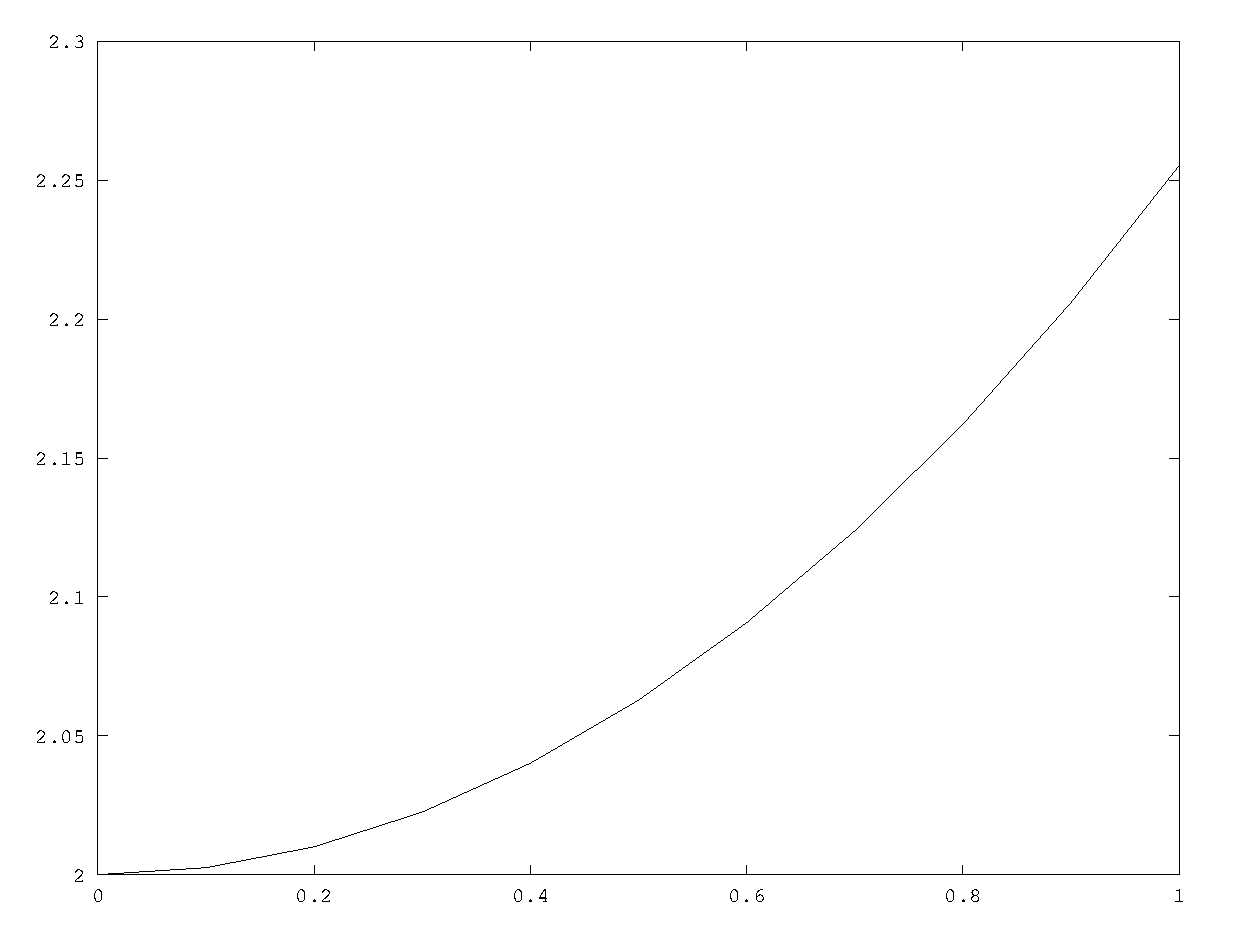
\includegraphics[width=\columnwidth]{g1}}
\end{mybox}
\vspace{10px}
\end{wrapfigure}

Isto é a famosa função \emph{catenária}. Os constantes $a$, $C_1$
e $C_2$ são os parâmetros que, em casos particulares, podemos encontrar
explicitamente. Vamos fazê-lo com a curva da figura
\ref{fig:1}. Supusemos que a linha é tangente em
$x=0$. Isso significa que em $x=0$, $dy/dx=0$. Como a equação
(\ref{eq:5}) dá que
\begin{equation}
  \label{eq:1}
  \frac{dy}{dx}=\senh\Big(\frac{x-C_1}{a}\Big),
\end{equation}
então em $x=0$, $\senh((0-C_1)(a))=0$. Portanto $C_1=0$. Se
adicionalmente a altura do poste à esquerda fosse exatamente
$h$, obtemos, que em $x=0$, o valor de $y$ é $h$. Então, da
equação (\ref{eq:5}) temos que $a+C_2=h$. Portanto a solução
é
\begin{equation}
  \label{eq:2}
  e = a \cosh(x/a) + h-a.
\end{equation}
É bastante comum supor que $a=h$. Então a solução tem a
forma
\begin{equation}
  \label{eq:3}
  e = h \cosh(x/h).
\end{equation}
Na figura \ref{fig:15} apresentamos vários gráficos desta função para
distintos $h$.


Mas, se adicionalmente conhecermos a altura do segundo poste, poderíamos
experimentar a encontrar o verdadeiro valor do parâmetro $a$ em
(\ref{eq:2}). Vamos supor, então, que a altura no ponto $x=x_2$ é
igual a $y_2$, isto é, em $x=x_2$, $y=y_2$. Portanto, a equação
que temos que resolver é
\begin{displaymath}
  e_2 = a \cosh(x_2/a) + h-a.
\end{displaymath}
Infelizmente, a solução desta equação não é
transcendental. Isso significa que não podemos expressá-la utilizando
funções elementares. Por isso, necessitamos utilizar umas ferramentas
computacionais para encontrar o parâmetro $a$ em casos
particulares e vamos explicá-lo depois.




\section{Longitude da catenária}

Se tivermos uma linha de longitude $l$ suspensa entre dois postes, qual
é a fórmula da catenária que forma a linha?  Portanto, isto deveria
ser fácil. Temos a fórmula geral~(\ref{eq:5}) que tem 3
incógnitas $a$, $C_1$ e $C_2$. As posições dos postes e uma
equação da longitude iria dar três equações. Ter três
equações deveria ser suficiente para encontrar três incógnitas. E
é. Portanto, agora o nosso objetivo é encontrar esta fórmula da
longitude da linha que necessitamos.


Provavelmente, num curso de cálculo ensinaram-lhe o seguinte. Seja
$\gamma$ uma curva dada pelo gráfico da função $y=f(x)$ para
$x\in [a,b]$. Então, a longitude $l$ da curva é
\begin{equation}
  \label{eq:6}
  l=\int_{x_1}^{x_2} \sqrt{1+(f'(x))^2}dx=\int_{x_1}^{x_2} \sqrt{1+\Big(\frac{dy}{dx}\Big)^2}dx.
\end{equation}
Desta fórmula vem a equação (\ref{eq:4}). De facto, definimos
uma variável $l$ como a longitude de $\gamma$ entre $x_1$ a $x$, isto é,
\begin{equation}
  \label{eq:10}
  l=\int_{x_1}^x \sqrt{1+\Big(\frac{dy}{dx}\Big)^2}dx.
\end{equation}
Derivando ambos os lados relativamente a $x$ e utilizando o Teorema
Fundamental de Cálculo, obtemos (\ref{eq:4}).

Agora utilizando (\ref{eq:1}), podemos encontrar a fórmula para $l$
entre $x_1$ a $x_2$. De facto
\begin{displaymath}
  l=\int_{x_1}^{x_2} \sqrt{1+\senh^2\Big(\frac{x-C_1}{a}\Big)}dx
  =\int_{x_1}^{x_2} \cosh\Big(\frac{x-C_1}{a}\Big)dx
\end{displaymath}
Então
\begin{equation}
  \label{eq:11}
  \boxed{l=a\senh\Big(\frac{x_2-C_1}{a}\Big)-a\senh\Big(\frac{x_1-C_1}{a}\Big)}
\end{equation}
e isto é a longitude.

\section{Caso geral}

Como já temos a fórmula para a longitude da linha (\ref{eq:11}),
podemos voltar ao nosso problema que foi colocado na secção
anterior. Vamos procurar a fórmula da catenária, quando tivermos
dado os pontos de fixação e a longitude da linha.


\begin{wrapfigure}{r}{0.5\textwidth}
  \vspace{-0.5cm}
  \begin{figurebox}
  \centering
  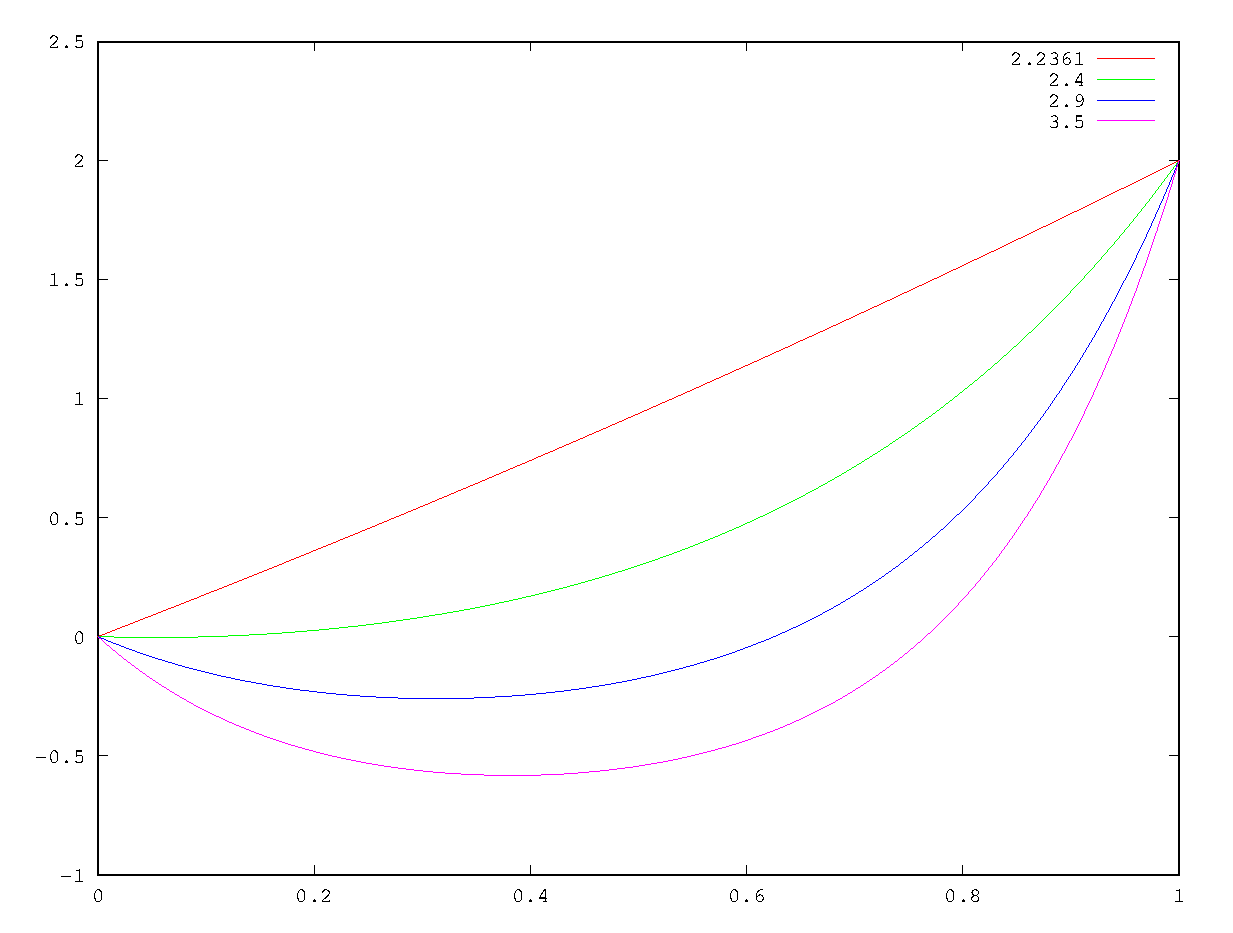
\includegraphics[width=\textwidth]{catenarias12}
  \caption{Linhas com diferentes longitudes.}
  \label{fig:4}
\end{figurebox}
\vspace{-2cm}
\end{wrapfigure}


Vamos supor que a linha está suspensa do lado direito no ponto
$(x_1,y_1)$. Então, da equação (\ref{eq:5}) temos que
\begin{displaymath}
  y_1=a\cosh\Big(\frac{x_1-C_1}{a}\Big) + C_2.
\end{displaymath}
Como do lado esquerdo o ponto denotamos por $(x_2,y_2)$, então
temos a segunda equação
\begin{displaymath}
  y_2=a\cosh\Big(\frac{x_2-C_1}{a}\Big) + C_2.
\end{displaymath}
Se adicionalmente denotamos a longitude da linha por $l$, utilizando
\eqref{eq:11} temos o seguinte sistema de equações
\begin{equation}
  \label{eq:12}
  \left\{
    \begin{array}{l}
      y_1=a\cosh\Big(\frac{x_1-C_1}{a}\Big) + C_2,\\
      y_2=a\cosh\Big(\frac{x_2-C_1}{a}\Big) + C_2,\\
      l=a\senh\Big(\frac{x_2-C_1}{a}\Big) - a\senh\Big(-\frac{C_1}{a}\Big).
    \end{array}
\right.
\end{equation}
Isto é um sistema que, em geral, não se pode resolver simbolicamente,
isto é a solução transcendental. Por isso, temos que utilizar
ferramentas computacionais, neste caso o programa livre
\Octave. Claramente, temos que transformar o nosso problema num outro que o computador pode entender. Vamos explicar como o fazemos.

Primeiro, vamos utilizar o comando \verb|fsolve|. Este comando
permite-nos encontrar zeros de uma função ou funções. Em primeiro lugar, para não
repetir a mesma fórmula várias vezes definimos uma função
\begin{displaymath}
  \cata(x,a) = a_1\Big(\cosh\big(\frac{x-a_2}{a_1}\big)\Big)+a_3.
\end{displaymath}


Isto é a fórmula de catenária \eqref{eq:5} mas alterámos a
notação. A variável $a$ é agora um vetor $(a_1,a_2,a_3)$ em que
$a_1$ corresponde ao parâmetro $a$ de \eqref{eq:5}, $a_2$ ao parâmetro
$C_1$ e $a_3$ ao $C_2$. Agora, com esta mudança, é muito fácil escrever esta função em \Octave. Escrevemos
simplesmente o seguinte.
\begin{octavebox}
\begin{verbatim}
function f = cata(x,a)
  f = a(1)*(cosh((x-a(2))/a(1)))+a(3);
endfunction
\end{verbatim}
\end{octavebox}

Fazemos o mesmo com a fórmula \eqref{eq:11} da longitude da
catenária. Escrevemo-la na forma
\begin{displaymath}
  \lCata(x_1,x_2,a)= a_1\Big(\senh\big(\frac{x_2-a_2}{a_1}\big) - \senh(\frac{x_1-a_2}{a_1})\Big),
\end{displaymath}
e em \Octave
\begin{octavebox}
\begin{verbatim}
function f = lCata(x1,x2,a)
  f = a(1)*(sinh((x2-a(2))/a(1))-sinh((x1-a(2))/a(1)));
endfunction
\end{verbatim}
\end{octavebox}

\begin{wrapfigure}{r}{0.4\textwidth}
  \vspace{-10px}
  \begin{figurebox}
    Nas definições de \Octave\ das funções \verb|cata|,
    \verb|lCata| e \verb|sistema1| o parâmetro \verb|a| é um vetor
    coluna. Por exemplo, se a nossa catenária tiver a fórmula
    \begin{displaymath}
      f(x) =  2\Big(\cosh\big(\frac{x-1}{2}\big)\Big)+5,
    \end{displaymath}
    então os parâmetros $a_1$, $a_2$ e $a_3$ são respetivamente
    igual a $2$, $1$ e $5$. Portanto, para calcular o valor da
    função no ponto $x= 3$ em otave escrevemos o seguinte.
    \begin{octavebox}
\begin{verbatim}
a=[2;1;5];
cata(3,a)
\end{verbatim}
    \end{octavebox}
    o resultado é
    \begin{octavebox}
\begin{verbatim}
ans =  8.0862
\end{verbatim}
    \end{octavebox}
  \end{figurebox}
  \vspace{-200px}
\end{wrapfigure}

Agora o sistema \eqref{eq:12} vamos reescrevê-lo na forma

\begin{octaveboxI}
\begin{verbatim}
 function f=sistema1(x1,y1,x2,y2,l,a)
   f(1) = y1 - cata(x1,a);
   f(2) = y2 - cata(x2,a);
   f(3) = l - lCata(x1,x2,a);
 endfunction
\end{verbatim}
\end{octaveboxI}

Depois para encontrar os coeficientes $a_1, a_2$, $a_3$ (\verb|a(1)|,
\verb|a(2)|, \verb|a(3)| em \Octave) da fórmula da catenária com $x_1=0$, $y_1=1$, $x_2=1$, $y_2=1.5431$ e $l=1.1752$.
Escrevemos
\begin{octaveboxI}
{\small
\begin{verbatim}
 a0=[1; 1; 1];
 fsolve(@(a) sistema1(0,1,1,1.5431,1.1752,a),a0)
\end{verbatim}}
\end{octaveboxI}
\noindent em que \verb|a0=[1; 1; 1]| é uma condição inicial. O que obtemos é o seguinte.
\begin{octaveboxI}
\begin{verbatim}
 ans =

    1.0001e+00
   -8.8204e-05
   -1.3329e-04
\end{verbatim}
\end{octaveboxI}
que são os parâmetros perto de $a_1=1$, $a_2=0$ e $a_3=0$. Então, a fórmula de catenária neste caso é quase
\begin{displaymath}
  f(x)=\cosh(x).
\end{displaymath}
A figura \ref{fig:4} era feita utilizando este programa com distintos
$l$.

Utilizando \Octave\  podemos agora facilmente encontrar a fórmula da catenária que passa por três pontos $(x_1,y_1)$, $(x_2,y_2)$ e $(x_3,y_3)$ dados. Neste caso, temos o seguinte sistema de equações
\begin{displaymath}
  \left\{
    \begin{array}{l}
      y_1=a_1\cosh\Big(\frac{x_1-a_2}{a_1}\Big) + a_3,\\
      y_2=a_1\cosh\Big(\frac{x_2-a_2}{a_1}\Big) + a_3,\\
      y_3=a_1\cosh\Big(\frac{x_3-a_2}{a_1}\Big) + a_3.
    \end{array}
  \right.
\end{displaymath}
que em \Octave\ reescreve-se como
\begin{octavebox}
\begin{verbatim}
function f=sistema2(x1,y1,x2,y2,x3,y3,a)
  f(1) = y1 - cata(x1,a);
  f(2) = y2 - cata(x2,a);
  f(3) = y3 - cata(x3,a);
endfunction
\end{verbatim}
\end{octavebox}

\begin{wrapfigure}{r}{0.5\textwidth}
      \vspace{-10pt}
  \begin{figurebox}
      \centering
      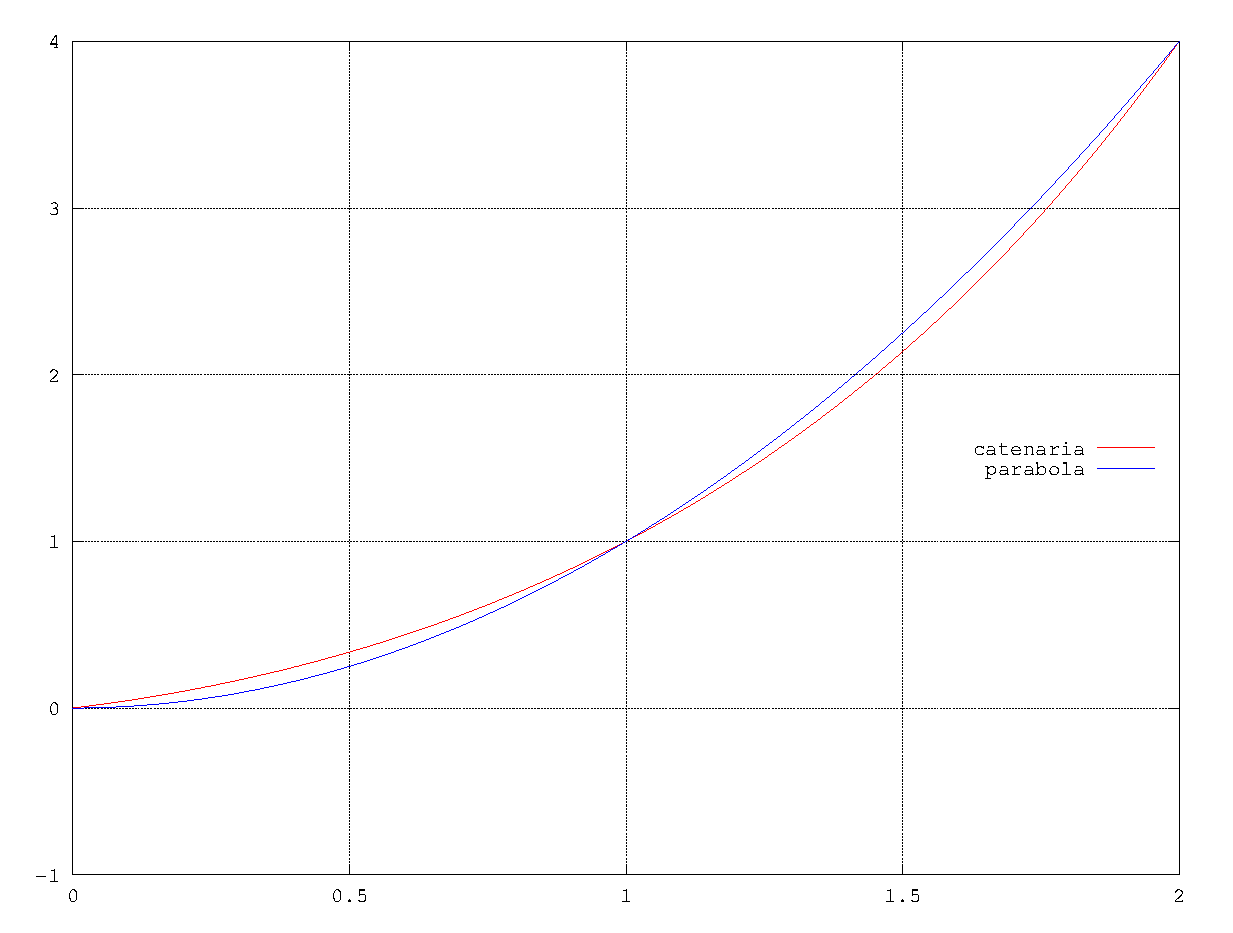
\includegraphics[width=\textwidth]{catenariaVsParabola}
      \caption{A única catenária e a única parábola que passam pelos
        pontos $(0,0)$, $(1,1)$ e $(2,4)$.}
    \label{fig:6}
  \end{figurebox}
    \vspace{-180pt}
\end{wrapfigure}

Com isto podemos, por exemplo, encontrar a única catenária que passa pelos pontos $(0,0)$, $(1,1)$ e $(2,4)$ escrevendo em \Octave\ o seguinte
\begin{octaveboxI}
\begin{verbatim}
 a0=[1; 1; 1];
 fsolve(@(a) sistema2(0,0,1,1,2,4,a),a0)
\end{verbatim}
\end{octaveboxI}
O resultado é
\begin{octaveboxI}
\begin{verbatim}
 ans =
    1.07724
   -0.42254
   -1.16118
\end{verbatim}
\end{octaveboxI}
Na figura \ref{fig:6} comparámos esta catenária com a parábola $y=x^2$.

\section{Fin}
\label{sec:fin}

A primeira pessoa que deu conta que a curva formada por uma
corrente não é parábola, era um jovem holandês, Christiaan Huygens. Sobre
a história deste descobrimento e a sua demonstração, pode ler-se em
\cite{Buk08}. Nós apresentámos uma demonstração moderna que
se pode encontrar em vários livros.

\bibliographystyle{plain}
\bibliography{catenaria}

\newpage
%%% Local Variables:
%%% mode: latex
%%% TeX-master: "matematicaseningenieria"
%%% End:
